\chapter{スペクトル画像を用いた非接触でのコーン指数推定の原理}
\thispagestyle{empty}
\label{ch:PrinciplesOfMethod}
\minitoc

\newpage
%%%%%%%%%%%%%%%%%%%%%%%%%%%%%%%%%%%%%%%%%%%%%%%%%%%%%%%%%%%%%%%%%%%%%%%%%%%%%%%

%==============================================================================
\section{はじめに}

本章では,非接触での走破性判定のために本研究で提案した,スペクトル画像を用いたコーン指数推定で利用する原理の詳細について解説する.

まず,\ref{sec:PrimciplesOfConeindexEstimation}節においては,
走破性を示す指標であるコーン指数を,土の他の性質を示す指標から推定する際に利用する原理について述べる.
本研究では,建設機械の走破性が,土の基礎的な性質に大きく影響されることを利用し,
コーン指数を,
% 土の基礎的な性質を示す
土の種類と含水比から推定する.

% "土の種類"という単語と"含水比"という単語を用いる
\ref{sec:SpectrumAndMaterialRelationship}節においては,
コーン指数を推定するために使用する土の種類と含水比を,非接触で推定する際に利用する原理について述べる.
本研究では,物質の種類と状態によって分光反射率スペクトルが変化することを利用し,
分光反射率スペクトルを用いて土の種類と含水比を推定する.
% 本研究では,土の種類と含水比を非接触で推定することで非接触での走破性判定を達成する.

\ref{sec:SpectrumFromSpectralImage}節においては,
分光反射率スペクトルをスペクトル画像から取得する手法の詳細について述べる.
本研究では,建設機械が通れる程度の面積の分光反射率スペクトルを取得するために,
広い面積の分光反射率スペクトルを取得できるスペクトル画像を用いる.

最後に,\ref{sec:Ground}節においては,
本研究で走破性判定の対象とする一般的な地盤について解説する.
次に,画像を用いることによって,
地盤の深い部分の土の情報を使用せずに表面の土の情報のみを使用して推定したコーン指数を
用いて判定した走破性の有効性について議論する.
% "地盤"と"土"という単語を使い分ける

\newpage


%==============================================================================
\section{土質パラメータによるコーン指数推定の原理}
\label{sec:PrimciplesOfConeindexEstimation}

\subsection{土質パラメータ}
\label{ssec:SoilParameters}

% まず最初に,土の性質を示す土質パラメータについて解説
土には様々な性質があり,その性質の程度を示すための指標が複数存在する.
例えば,土における植物の育ちやすさを示す指標としては土のpH値があり,
pH値が低い酸性の土では植物が育ちにくいことが知られている\cite{三枝1991}\cite{図子1993}.
% 土のpH値の測定方法,説明
% pH値が低い酸性の土では植物が育ちにくいことが知られている.
また,地震によって液状化が発生する際の液状化の激しさの程度を示す指標としては
地盤液状化指数があり,
地盤液状化指数が大きいほど液状化が発生した時の構造物への被害は大きなることが知られている\cite{龍岡1980}\cite{岩崎1980}\cite{浜田1986}.
% 地盤液状化指数の測定方法
% 一般的には地盤液状化指数が大きい地盤ほど
% 液状化が発生した時の構造物への被害は大きくなる.
その他にも,斜面の安定性などの様々な土の性質を示す指標が存在する\cite{三笠1964}.
このような土の性質の程度を示す指標のことを土質パラメータと言う\cite{山口1986}\cite{渡部2007}.
多くの土の性質は土の有する他の性質から影響を受けるため,土質パラメータも他の土質パラメータから大きな影響を受けることが多い\cite{太田1988}\cite{三隅1992}.
このような土質パラメータのうちの1つに,走破性の高さを示す指標であるコーン指数という土質パラメータが存在する.

\subsection{コーン指数}
\label{ssec:Coneindex}

% そのうちの1つであるコーン指数が,走破性の高さを示す指標であることを述べた
\ref{ssec:SoilParameters}項で述べたように,土質パラメータのうちの1つに,不整地の上を走る車両の走破性の高さを示すコーン指数という土質パラメータが存在する.
コーン指数は,1948年にアメリカ陸軍工兵隊で開発されたコーンペネトロメータという器具を使用して測定する指標である\cite{WES1948}\cite{Perumpral1987}.
当時開発されたコーンペネトロメータは,長さ91.4cm, 直径0.95cmのシャフトに,先端角$30^\circ$,底面の面積が1.61$\rm cm^2$の円錐状のコーンを
つけ,シャフトの円錐状のコーンをつけた側とは反対側に土の抵抗を測定するためのゲージとハンドルを搭載していた.
使用方法は,
最初にゲージの値を0に合わせた後,
シャフトを円錐状のコーンの付いた方から地面に挿入し,その際の抵抗を上部のゲージで読み取って,
その値からシャフトの先端についているコーンの底面の面積を割り,一定の係数をかけることでコーン指数が算出される.
コーンペネトロメータは持ち運びが容易なため,
走破性を判定する以外にも様々な用途に使用されるようになり,
その用途に合わせてコーンペネトロメータの寸法も変化し,多くの派生型が作成された\cite{Hendrick1969}\cite{Prather1970}.
% 派生型の説明 \cite{Perumpral1987}から孫引き
\ref{ssec:SoilParameters}項で述べたように,多くの土の性質と同じく走破性は土の有する他の性質から影響を受けるため,
走破性を示す指標であるコーン指数も他の土質パラメータから大きな影響を受ける.

\subsection{コーン指数以外の土質パラメータからのコーン指数の推定}
\label{ssec:ConeindexEstimation}

走破性に影響を与える他の土の性質として,% 土の性質は走破性,土質パラメータはコーン指数に影響を与える
土の粒子の材質や直径の分布,形,表面の粗さ,土に含まれる水の量などの基礎的な土の性質を挙げることができる\cite{小田1971}\cite{Okello1991}\cite{Shoop1993}\cite{Flores2014}.
それらを示す指標としては,土の粒子の鉱物組成,有機物含有量,粒度分布,球形率,含水比が挙げられる.% それぞれの指標の説明 "定量化した"ではなく"示す"指標という表現に統一
% それぞれの土質パラメータの測定方法を引用
従って,土質パラメータの土の粒子の鉱物組成,有機物含有量,粒度分布,球形率,含水比は
走破性の指標であるコーン指数に大きな影響を与える\cite{Collins1971}.% 引用
つまり,これらの基礎的な土の性質を示す土質パラメータが分かれば,コーン指数も一意に決まる\cite{Ayers1982}\cite{Jenkins1985}\cite{Elbanna1987}\cite{Mulhearn2001}.

上記の基礎的な土の性質を示す土質パラメータのうち,外部の状況に左右されない土に固有の土質パラメータである土の粒子の鉱物組成,有機物含有量,粒度分布,球形率が
同じ土を同じ種類の土であると定義すると,
コーン指数に大きな影響を与える残りの土質パラメータは含水比のみとなる.
従って,
土の種類と含水比が分かれば,コーン指数は一意に決まる.

そこで本研究では,
% 上記で述べた土の種類と含水比のコーン指数との関係を利用することによって,
上記で述べたコーン指数と基礎的な土の性質を示す土質パラメータの関係を利用することによって,
土の種類と含水比から
コーン指数の推定を行う.

\clearpage


\section{分光反射率スペクトルでの土質パラメータ推定の原理}
\label{sec:SpectrumAndMaterialRelationship}

\subsection{分光反射率スペクトル}
\label{ssec:Spectrum}

物質は,その分子や原子の構造,または物質を構成する微粒子の大きさや形,表面の凹凸によって,
光の波長ごとの反射,散乱,吸収,そして放射の度合いが異なる\cite{Shaw2002}\cite{Shaw2003}.
従って,物質の種類と状態によって,分光反射率スペクトルが異なる.
分光反射率スペクトルとは,下の式のように,物質に入射してくる光のエネルギーに対して,
その物質が反射した光のエネルギーの割合を波長ごとに並べたものである.% 引用
分光反射率を示す式は,
\begin{eqnarray}
\rho(\lambda) = \frac{L_s(\lambda)}{L_i(\lambda)}\label{eq:reflectance_spectrum_caliculation}
\end{eqnarray}
となる.\mbox{式(\ref{eq:reflectance_spectrum_caliculation})}において,$\rho(\lambda)$は物質の分光反射率を,
$L_s(\lambda)$は物質が反射する光の強さを,そして$L_i(\lambda)$は物質に入射する光の強さをそれぞれ示す.
また,$\lambda$は波長を示し,$\rho(\lambda)$,$L_s(\lambda)$,$L_i(\lambda)$は波長の関数である.

この分光反射率スペクトルを使用することによって,物質の種類の識別と状態の推定を非接触で行うことが可能である.
例えば,化学や物理学の分野では分光反射率スペクトルが物質の識別などに使用されている\cite{長田2004}.
% もっと具体的な例を追加

% \mbox{式(\ref{eq:r})}

\subsection{非接触での土質パラメータの推定}
\label{ssec:NonContactEstimation}

分光反射率スペクトルを用いて土質パラメータを非接触に推定することも可能である.
例えば,土のpH値の推定や,含水比の推定などに使用されている\cite{Ben-Dor2002}\cite{Rossel2006}.%\cite{McCarty2002}\cite{Cozzolino2003}.% 引用ごとの例を解説
また,土の種類に含めた,外部の状況に左右されない土に固有の土質パラメータである土の粒子の鉱物組成,有機物含有量を推定することも可能である\cite{Ben-Dor1995}\cite{Janik1998}.
さらに,粒度分布も分光反射率スペクトルに影響を与えることが分かっている\cite{小嶋1996}.
従って,分光反射率スペクトルを用いて,コーン指数に大きな影響を与える土の種類と含水比を推定することが期待できる\cite{小川1989}\cite{Jia2017}.
% "可能である"と"できる"を使用

\clearpage


\section{スペクトル画像からの分光反射率スペクトルの取得}
\label{sec:SpectrumFromSpectralImage}

\subsection{スペクトル画像}
\label{ssec:SpectralImage}

\ref{sec:SpectrumAndMaterialRelationship}節で述べた通り,本研究では,分光反射率スペクトルを用いることによって,
土の種類の識別と含水比の推定を非接触に行う.
この土の種類と含水比を用いてコーン指数を推定することによって,建設機械のための走破性の判定を非接触に行うことが可能になると期待できる.

建設機械の走破性を判定するためには,対象となる建設機械が走行できる程広い面積の土のコーン指数を推定する必要がある.
それ程広い面積のコーン指数を推定するためには,
% コーン指数に大きな影響を与える土質パラメータも
コーン指数に大きく影響する土の種類の識別と含水比の推定に用いる分光反射率スペクトルを
広範囲で測定しなければならない.
% しかし,これまでの分光反射率スペクトルの測定の多くはスポット推定であり,建設機械が走行する面積と比較すると
% 非常に狭い面積の分光反射率スペクトルしか測定できない\cite{長田2004}\cite{田代2013}\cite{蔦2002}.
そこで,本研究では,十分広い面積の分光反射率スペクトルを取得できるスペクトル画像を使用する\cite{蔦2002}\cite{長田2004}\cite{田代2013}.

スペクトル画像とは,撮影した対象物から反射してきたカメラへの入射光を分光させることによって,複数の波長帯の光の強さを記録した画像である\cite{中野1996}\cite{眞鍋1996}\cite{Tominaga1999}.
一般的なRGB画像がR,G,Bの3波長帯の光の強さを記録した画像であるのに対し,スペクトル画像の波長帯の数は4以上であり,多い場合には数百に及ぶ\cite{Goetz1985}.% 例を追加
% スペクトル画像のイメージを図\ref{fig:spectral_image}に示す.
一般的なRGB画像とスペクトル画像を,それぞれ図\ref{fig:RGBimage_spectralimage_comparison}(a)および(b)に示す.
図\ref{fig:RGBimage_spectralimage_comparison}(a)および(b)において,x, y軸方向は空間方向の広さを示し,
z軸方向は波長方向の長さを示す.
また,図\ref{fig:RGBimage_spectralimage_comparison}(a)および(b)において,z軸方向に積層された各画像が,分光されたそれぞれの波長帯を示す.
従って,一般的なRGB画像を示す図\ref{fig:RGBimage_spectralimage_comparison}(a)においては,z軸方向に積層された画像の枚数がR,G,Bの3枚となり,
一方スペクトル画像を示す図\ref{fig:RGBimage_spectralimage_comparison}(b)においては,z軸方向に積層された画像の枚数が4枚以上となる.

% 従って,z軸方向に積層された画像の枚数が,入射光を分光させて光の強さを記録した波長帯の数を示す.

% \begin{figure}[p]
% 	\begin{center}
% 	\centering
% 	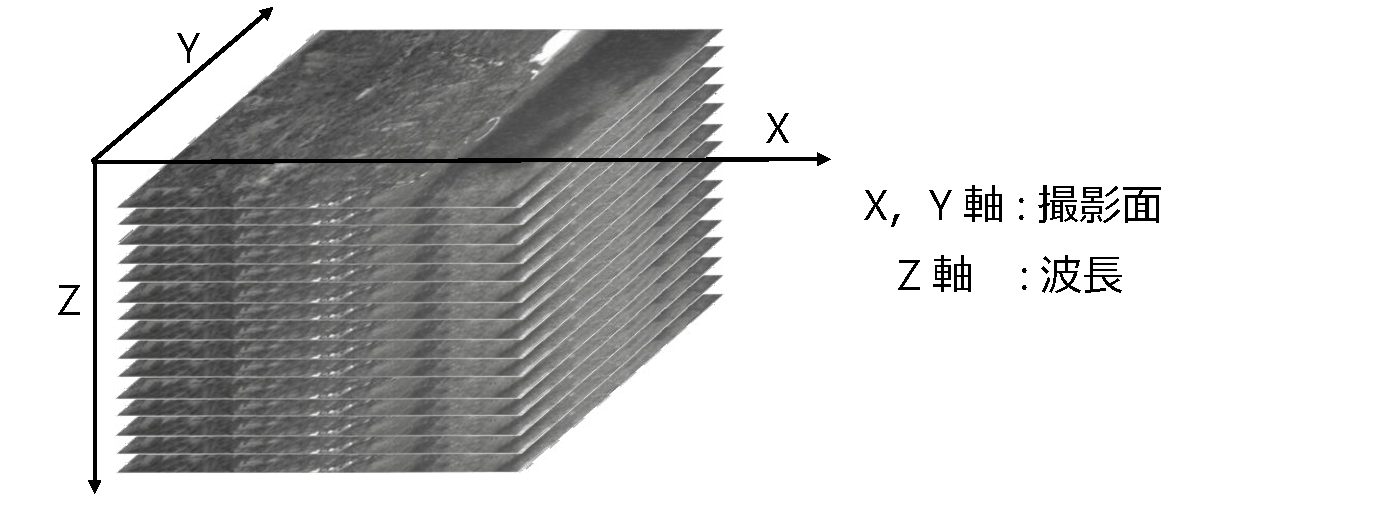
\includegraphics[width=11cm]{./Ch2_PrinciplesOfMethod/Fig/spectralimage_compressed.pdf}
% 	\caption{スペクトル画像}\label{fig:spectral_image}
% 	\end{center}
% \end{figure}

\begin{figure}[p]
	\begin{center}

		% \begin{minipage}[b]{0.9\linewidth}
		% \centering
		% 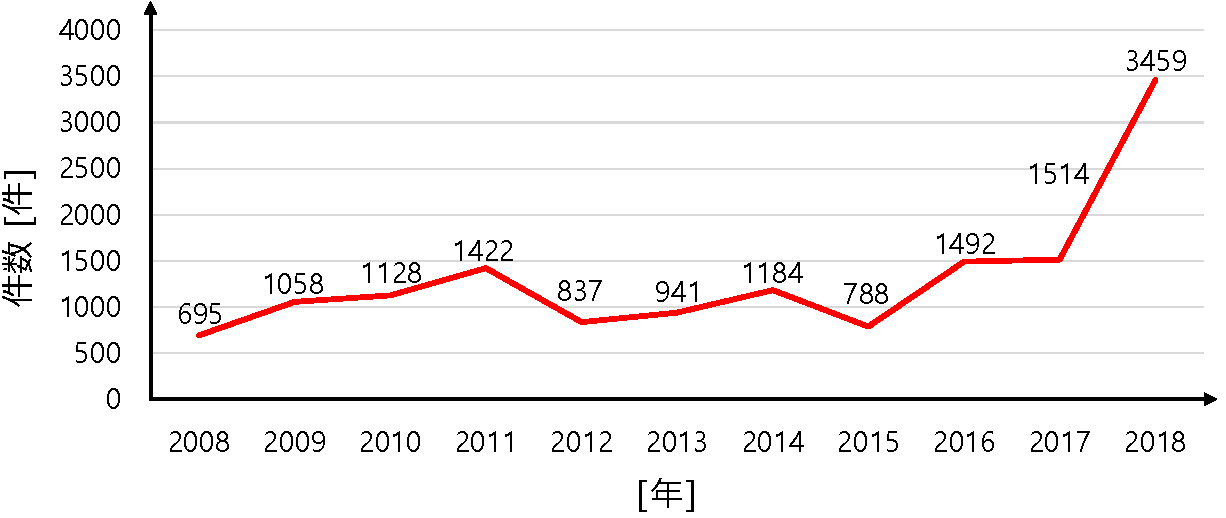
\includegraphics[width=12cm]{./Ch1_Introduction/Ch1_Fig/土砂災害発生件数.pdf}
		% \vspace{-3mm}
		% \caption*{(a)土砂災害発生件数}
		% \end{minipage}\\

		\begin{minipage}[b]{\linewidth}
		\centering
		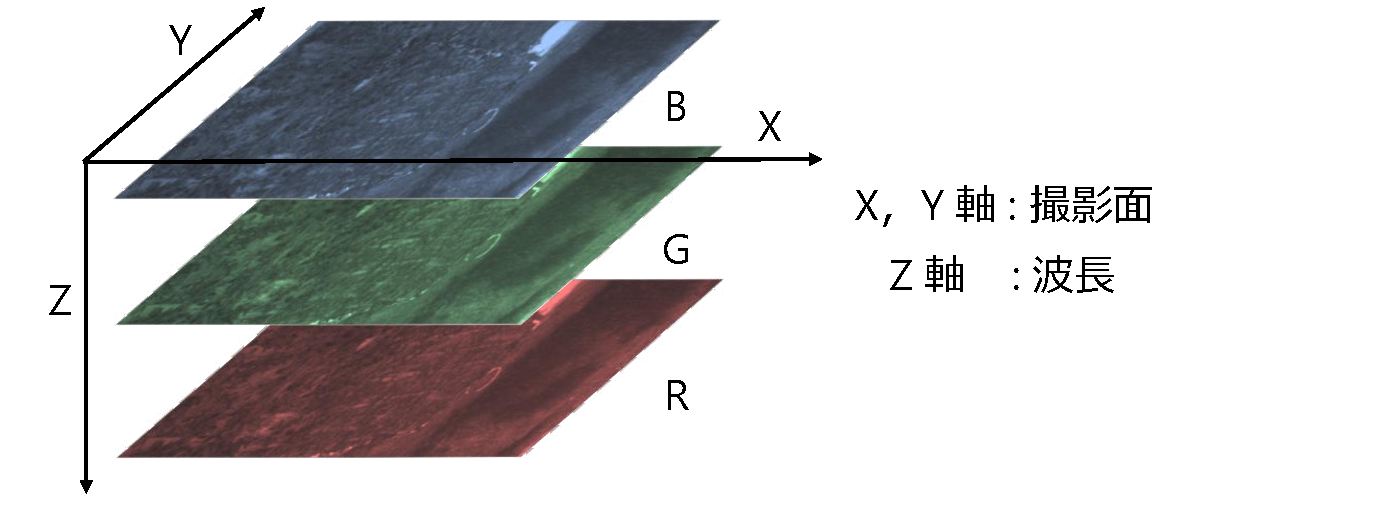
\includegraphics[width=12.5cm]{./Ch2_PrinciplesOfMethod/Fig/RGBimage_compressed.pdf}
		\vspace{-2mm}
		\caption*{(a)一般的なRGB画像} 
		\vspace{1cm} % 上下の画像の間を調整
		\end{minipage}\\

		\begin{minipage}[b]{\linewidth}
		\centering
		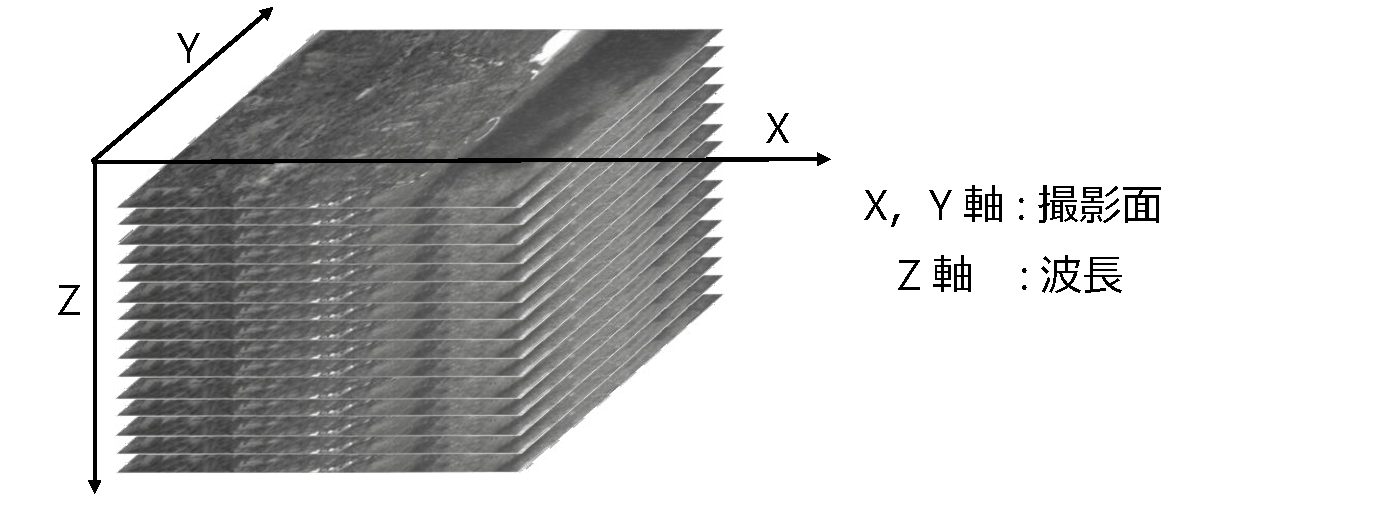
\includegraphics[width=12.5cm]{./Ch2_PrinciplesOfMethod/Fig/spectralimage_compressed.pdf}
		\vspace{-2mm}
		\caption*{(b)スペクトル画像} 
		\end{minipage}
	
	\caption{一般的なRGB画像とスペクトル画像の比較}\label{fig:RGBimage_spectralimage_comparison}
	\end{center}
\end{figure}

% ハイパースペクトル画像・マルチスペクトル画像は具体的な方法 
% スペクトル画像全般は原理で説明

\clearpage

\subsection{分光反射率スペクトルの取得}
\label{ssec:SpectrumGet}

スペクトル画像は,波長帯ごとの分光反射率が分かっている物質を画像に入れるように撮影することで,画像に写りこんだその物質以外の物質の
各波長帯における分光反射率を算出することができる.
その各波長帯の分光反射率を波長順に並べることによって,画像中の物質の分光反射率スペクトルを取得することができる.% 引用

そこで,本研究では,
% 従って,
分光反射率が既知の校正用物質を含めて撮影したスペクトル画像から
スペクトル画像内に分布している校正用物質以外の分光反射率スペクトルを取得する.
% 本研究ではこのようにしてスペクトル画像から分光反射率スペクトルを取得する.

% 土の分光反射率スペクトルの例を示す

\clearpage

\section{本研究で対象とする地盤}
\label{sec:Ground}

スペクトル画像を用いて土を撮影し,
土の種類の識別と含水比の推定を
行う場合,土の表面のみの情報からコーン指数を推定することになる.
従って,スペクトル画像
を用いてコーン指数を推定する場合,
従来のコーンペネトロメータを用いた手法で利用してきた
土の深い部分の情報を利用することができず,
表面の土のコーン指数のみを推定することになる.
しかし,一般的に,土は深いところにあるほど上の土の質量が増加するため
圧密により固くなる
ことが多い\cite{森本1975}\cite{高田1983}.
また,同じ場所ならば,基本的には表面にある土も深いところにある土も同じ種類の土である.% 引用
土の種類が同じならば圧密による固さの度合いは上に積層した土の質量のみに依存するため,
深いところにある土ほど固くなる.
そこで,本研究では,上記で述べたような一般的にみられる,
土の表面と深部における土の種類が同じであり,
深くなるにつれて土の硬さが単調に増加する地盤を対象とする.
% 深部にある土ほど固くなっている地盤を対象とする.
% 本研究で対象とする一般的な地盤におけるコーン指数と深さの関係を
% 図\ref{fig:relationship_between_coneindex_and_depth}に示す.
% 図\ref{fig:relationship_between_coneindex_and_depth}のグラフにおいて,
% 縦軸は土の深さ,横軸はコーン指数を示す.
% この図\ref{fig:relationship_between_coneindex_and_depth}のグラフより,
% 本研究で対象とする地盤の土は,土の深さとコーン指数が比例することが分かる.


% \begin{figure}[b]
% 	\begin{center}
% 	\centering
% 	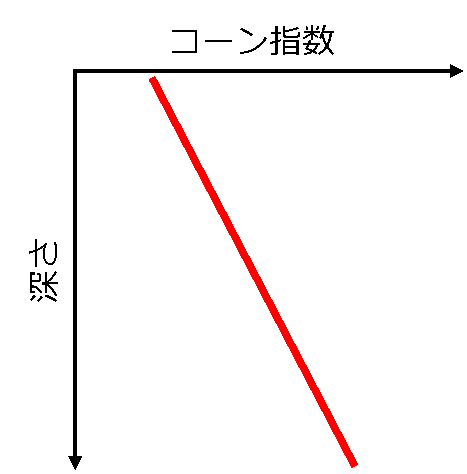
\includegraphics[width=4.5cm]{./Ch2_PrinciplesOfMethod/Fig/relationship_between_coneindex_and_depth_compressed.pdf}
% 	\caption{コーン指数と土の深さの関係}\label{fig:relationship_between_coneindex_and_depth}
% 	\end{center}
% \end{figure}

以上より,一番上にある一番軟らかい土のコーン指数が建設機械の重量に耐えられるならば,
深い部分にある固い土のコーン指数も当然建設機械の重量に耐えるため,
土の表面にある一番軟らかい土の情報のみを利用して推定したコーン指数を用いた
非接触での走破性判定は有効である.

\clearpage

\section{ハイパースペクトル画像とマルチスペクトル画像}
\label{sec:HyperAndMultiImages}

本研究では,スペクトル画像を用いて土の種類の識別と含水比の推定を行う.
具体的には,土の種類の識別には,波長幅の短い波長帯を多数取得できるハイパースペクトル画像を用い,
含水比の推定には,含水比の増加に伴って分光反射率が減少する近赤外の光を1つの波長帯で取得できる
マルチスペクトル画像を用いる.

ハイパースペクトル画像とは,
スペクトル画像の中でも,入射光を分光して記録する波長帯の数が非常に多いスペクトル画像である\cite{横矢2014}.
土の種類の識別の際には,水分子が吸収しない波長における分光反射率スペクトルの詳細な形状が必要になるため,
ハイパースペクトル画像を用いる.
ハイパースペクトル画像を用いた土の種類の識別の詳細については,第\ref{ch:SoilTypeDiscrimination}章で解説する.

一方,マルチスペクトル画像とは,スペクトル画像のなかでも分光させる波長帯の数が少ない画像である.
近赤外の光の分光反射率を用いて含水比を推定するためには,
近赤外の幅広い範囲の光を1つの波長帯として取得するスペクトル画像を用いる必要がある.
そのため,含水比の推定の際には,スペクトル画像のなかでも,入射光を分光させる波長帯の数が少なく,1つの波長帯当たりの波長幅を大きくすることが
できるマルチスペクトル画像を用いる.
マルチスペクトル画像を用いた含水比の推定の詳細については,第\ref{ch:WaterContentEstimation}章で解説する.

\clearpage

\section{おわりに}

本章では,スペクトル画像を用いて土の種類と含水比を推定し,その2つからコーン指数を推定する手法の原理について述べた.

まず,\ref{sec:PrimciplesOfConeindexEstimation}節において,
% 土の基礎的な性質を示す土質パラメータ
土の種類と含水比からコーン指数を推定する手法の原理の詳細について述べた.% "建設機械の走破性"
コーン指数は,土の基礎的な性質を示す土の粒子の鉱物組成,有機物含有量,粒度分布,球形率,含水比に大きく影響される.
本研究ではこれを利用し,外部の状況に左右されない,土に固有の土質パラメータである土の粒子の鉱物組成,有機物含有量,粒度分布,球形率
をひとまとめにした土の種類と,それに該当せず外部の状況によって変化する含水比の2つからコーン指数を推定する.

次に,\ref{sec:SpectrumAndMaterialRelationship}節において,
分光反射率スペクトルを用いて土の種類の識別と含水比の推定を行う手法の原理について述べた.
分光反射率スペクトルは物質の種類と状態によって変化するため,
物質の種類と状態を分光反射率スペクトルを用いて推定することが可能である.
そこで,本研究でも,分光反射率スペクトルを用いることによって,
土の種類の識別と含水比の推定を非接触に行う.
分光反射率スペクトルを用いて識別した土の種類と推定した含水比を用いてコーン指数を推定することによって,
非接触での建設機械の走破性判定を行う.

次に,\ref{sec:SpectrumFromSpectralImage}節において,
分光反射率スペクトルを取得するためのスペクトル画像について述べた.
建設機械の走破性を判定するためには,建設機械の走行面積以上の
広さのコーン指数を推定する必要があるため,広い面積の土の種類と含水比を
推定する必要があり,その範囲における分光反射率スペクトルを取得する必要がある.
従って,本研究では,
広い面積の分光反射率スペクトルを取得できるスペクトル画像を用いる.

また,\ref{sec:Ground}節において,
本研究で対象とする一般的な地盤について解説した後,
画像を用いて非接触での走破性判定を行うにあたり,
土の表面の情報のみを利用することについての議論を行った.
その議論において,本研究で対象とする一般的な地盤においては,
画像を用いて土の表面の情報のみを利用しても,
走破性の判定は
可能であることを示した.

最後に,\ref{sec:HyperAndMultiImages}節において,
本研究において使用する,ハイパースペクトル画像とマルチスペクトル画像の違いと
それぞれの画像を使い分けた理由を簡単に解説した.

% \newpage

%%%%%%%%%%%%%%%%%%%%%%%%%%%%%%%%%%%%%%%%%%%%%%%%%%%%%%%%%%%%%%%%%%%%%%%%%%%%%%%
%%% Local Variables:
%%% mode: katex
%%% TeX-master: "../thesis"
%%% End:
